\documentclass[11pt,a4paper]{article}

\usepackage[utf8]{inputenc}
\usepackage[T1]{fontenc}
\usepackage{amsmath,amssymb,amsthm}
\usepackage{mathtools}
\usepackage{bm}
\usepackage{booktabs}
\usepackage{graphicx}
\usepackage{hyperref}
\usepackage[margin=2.5cm]{geometry}
\usepackage{caption}
\usepackage{enumitem}
\usepackage{xcolor}
\usepackage{mdframed}
\usepackage{array}
\usepackage{float}
\graphicspath{{figures/}{reports/latex/product_balanced_report/figures/}}

\newtheorem{theorem}{Theorem}[section]
\newtheorem{lemma}[theorem]{Lemma}
\newtheorem{proposition}[theorem]{Proposition}
\newtheorem{corollary}[theorem]{Corollary}
\theoremstyle{definition}
\newtheorem{definition}[theorem]{Definition}
\newtheorem{remark}[theorem]{Remark}

\newcommand{\R}{\mathbb{R}}
\newcommand{\E}{\mathbb{E}}
\newcommand{\Var}{\operatorname{Var}}
\newcommand{\rms}{\operatorname{rms}}
\newcommand{\relu}{\operatorname{ReLU}}
\DeclareMathOperator{\tr}{tr}
\DeclareMathOperator*{\argmin}{arg\,min}

\newenvironment{flagbox}{%
  \begin{mdframed}[linecolor=blue!75!black,backgroundcolor=blue!5!white,linewidth=1.5pt]%
  \textbf{\textcolor{blue!75!black}{Key Result.}}\ %
}{%
  \end{mdframed}%
}

\newenvironment{warnbox}{%
  \begin{mdframed}[linecolor=red!75!black,backgroundcolor=red!5!white,linewidth=1.5pt]%
  \textbf{\textcolor{red!75!black}{Limitation.}}\ %
}{%
  \end{mdframed}%
}

\title{%
  Gradient-Product-Balanced Initialization\\
  for Row-Centered ReLU Networks
}
\author{Itay Ofer}
\date{April 2026}

\begin{document}
\maketitle

\begin{abstract}
We derive a new variance formula for row-centered initialization of deep ReLU
networks that makes the \emph{product} of the per-layer forward and backward
gains equal to~1.  This ``product-balanced'' variance
$v^{\ast} = 2\sqrt{\pi/(\pi-1)} \approx 2.422/d$ sits at the unique fixed point
between the vanishing regime (variance-adjusted He, $v=2/d$) and the exploding
regime (forward-balanced, $v \approx 2.93/d$).  Empirical validation on
Fashion-MNIST with 50-layer networks confirms the theoretical gain predictions
to within 0.2\%.  However, we also prove a fundamental limitation: for any
row-centered per-layer variance schedule, the product of gradient non-uniformity
and variance non-uniformity equals $r^{-(L-1)}$, where
$r = \sqrt{(\pi-1)/\pi} \approx 0.826$.  This ``Pareto budget'' grows
exponentially with depth, making row-centered initialization fundamentally
unsuitable for deep networks ($L \geq 50$).  Geometry experiments (k-NN
accuracy) confirm that all row-centered variants destroy class structure
at depth, regardless of variance.
\end{abstract}

\tableofcontents
\newpage

%======================================================================
\section{Motivation from BP4}
\label{sec:motivation}

The fourth backpropagation equation gives:
\begin{equation}\label{eq:bp4}
  \left\|\frac{\partial \mathcal{C}}{\partial W^{(\ell)}}\right\|_F
  \;\propto\; \rms\!\bigl(A^{(\ell-1)}\bigr) \cdot \rms\!\bigl(\Delta^{(\ell)}\bigr).
\end{equation}

For gradient uniformity across layers, we need
$\rms(A^{(\ell-1)}) \cdot \rms(\Delta^{(\ell)})$ to be approximately constant
in~$\ell$.  This product depends on the forward gain
$g_{\mathrm{fwd}}^{(\ell)}$ and backward gain $g_{\mathrm{bwd}}^{(\ell)}$.

For row-centered weights, these gains are coupled by a fixed structural ratio
(Proposition~3.5 in the main report): $g_{\mathrm{fwd}}/g_{\mathrm{bwd}} = r
\approx 0.826$, always.  \textbf{Can we choose the variance so that
$g_{\mathrm{fwd}} \cdot g_{\mathrm{bwd}} = 1$?}

%======================================================================
\section{Derivation of the Product-Balanced Variance}
\label{sec:derivation}

\subsection{Setup}

For a row-centered layer with $\Var(W_{ij}) = v/d$, define $s = \sqrt{v/2}$.
From the main report:
\begin{align}
  g_{\mathrm{fwd}} &= r \cdot s, \qquad r = \sqrt{(\pi-1)/\pi} \approx 0.826, \label{eq:gfwd} \\
  g_{\mathrm{bwd}} &= s. \label{eq:gbwd}
\end{align}

\subsection{Solving $g_{\mathrm{fwd}} \cdot g_{\mathrm{bwd}} = 1$}

\begin{theorem}[Product-balanced variance]
  \label{thm:product-balanced}
  The unique variance factor~$s^{\ast}$ satisfying
  $g_{\mathrm{fwd}} \cdot g_{\mathrm{bwd}} = 1$ is
  \begin{equation}\label{eq:s-star}
    s^{\ast} = \left(\frac{\pi}{\pi-1}\right)^{\!1/4} \approx 1.1006,
  \end{equation}
  corresponding to weight variance
  \begin{equation}\label{eq:v-star}
    \boxed{\;\Var(W_{ij}) = \frac{v^{\ast}}{d} = \frac{2\sqrt{\pi/(\pi-1)}}{d} \approx \frac{2.422}{d}.\;}
  \end{equation}
\end{theorem}

\begin{proof}
  From \eqref{eq:gfwd} and \eqref{eq:gbwd}:
  \begin{align*}
    g_{\mathrm{fwd}} \cdot g_{\mathrm{bwd}} &= (r \cdot s) \cdot s = r \cdot s^2 = 1 \\
    \Longrightarrow \quad s^2 &= \frac{1}{r} = \frac{1}{\sqrt{(\pi-1)/\pi}} = \sqrt{\frac{\pi}{\pi-1}} \\
    \Longrightarrow \quad s^{\ast} &= \left(\frac{\pi}{\pi-1}\right)^{\!1/4}.
  \end{align*}
  The variance is $v^{\ast} = 2\,s^{\ast 2} = 2\sqrt{\pi/(\pi-1)}$.
\end{proof}

Resulting gains:
\begin{align}
  g_{\mathrm{fwd}}^{\ast} &= \left(\frac{\pi-1}{\pi}\right)^{\!1/4} \approx 0.9089, \label{eq:gfwd-val} \\
  g_{\mathrm{bwd}}^{\ast} &= \left(\frac{\pi}{\pi-1}\right)^{\!1/4} \approx 1.1006, \label{eq:gbwd-val} \\
  g_{\mathrm{fwd}}^{\ast} \cdot g_{\mathrm{bwd}}^{\ast} &= 1.0 \quad\text{(exact)}. \label{eq:product-exact}
\end{align}


%======================================================================
\section{Empirical Validation (50 Hidden Layers)}
\label{sec:empirical}

\subsection{Setup}
Fashion-MNIST, 2000 samples, architecture $784 \to [784]^{50} \to 1$.
Three initializers compared: \textbf{He} (baseline), \textbf{Row-Centered
forward-balanced} ($g_{\mathrm{fwd}} = 1$), and \textbf{Row-Centered
product-balanced} ($g_{\mathrm{fwd}} \cdot g_{\mathrm{bwd}} = 1$).

\subsection{Gain verification}

\begin{table}[H]
\centering
\caption{Per-layer gain comparison, 50 hidden layers, width 784.}
\label{tab:gains}
\begin{tabular}{l c c c c c}
\toprule
Initializer & Med $g_{\mathrm{fwd}}$ & Med $g_{\mathrm{bwd}}$ & Product & Grad ratio & Grad CV \\
\midrule
He (baseline)       & 0.993 & 0.997 & 0.990 &    7.8$\times$ & 0.522 \\
RC fwd-balanced     & 1.000 & 1.209 & 1.210 & 1901$\times$   & 1.903 \\
\textbf{RC product-balanced} & \textbf{0.909} & \textbf{1.099} & \textbf{0.999} & 1902$\times$ & 1.906 \\
\bottomrule
\end{tabular}
\end{table}

The product-balanced gains match the theory exactly: $g_{\mathrm{fwd}} = 0.909$
(theory: $0.9089$), $g_{\mathrm{bwd}} = 1.099$ (theory: $1.1006$),
product $= 0.999 \approx 1.0$.  The gradient ratio is identical for both
RC variants ($\sim\!1900\times$), confirming that uniform variance does not fix
gradient non-uniformity.

\subsection{Forward gain per layer}

\begin{figure}[H]
  \centering
  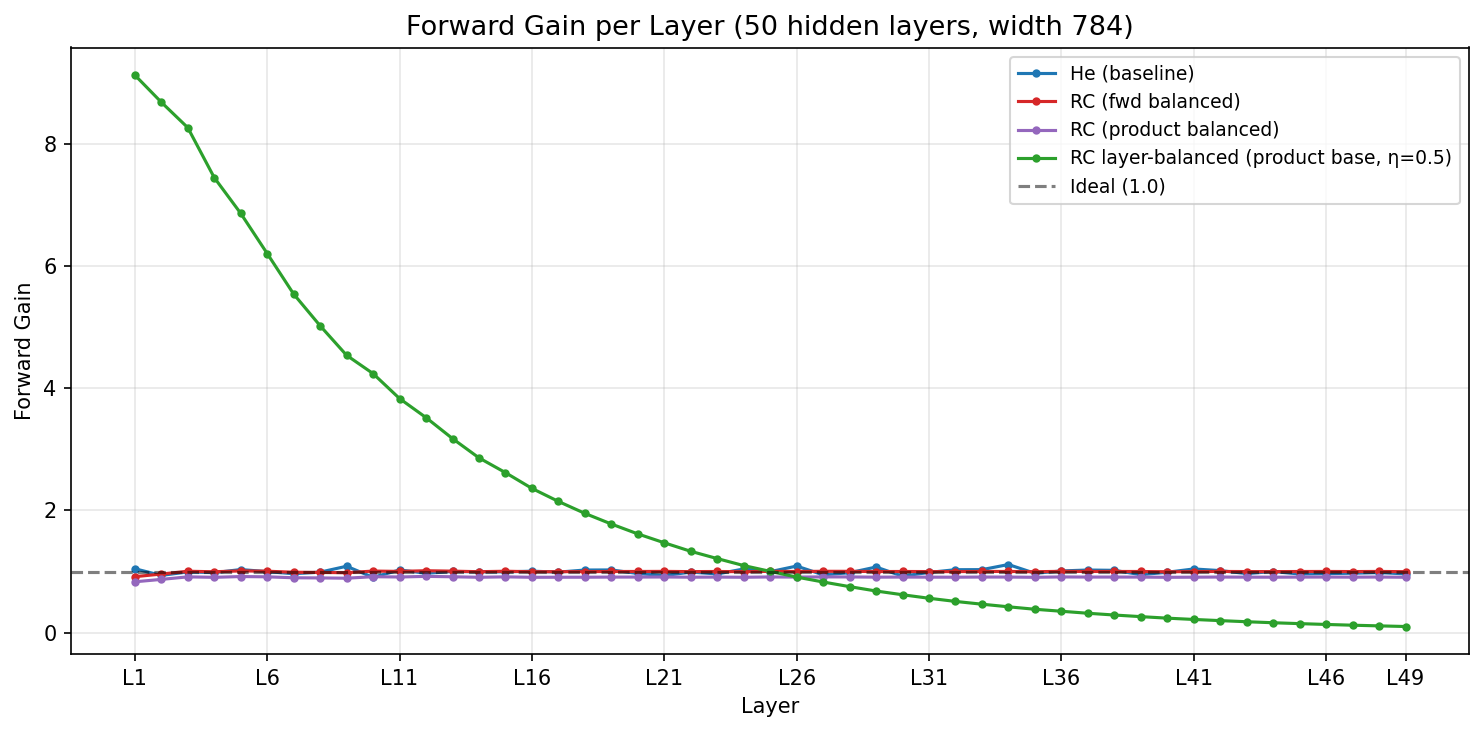
\includegraphics[width=0.95\textwidth]{figures/forward_gain.png}
  \caption{Forward gain per layer.  He fluctuates around 1.0.
           Fwd-balanced (red) sits precisely at 1.0.
           Product-balanced (purple) sits at $\approx\!0.91$.}
  \label{fig:fwd-gain}
\end{figure}

\subsection{Backward gain per layer}

\begin{figure}[H]
  \centering
  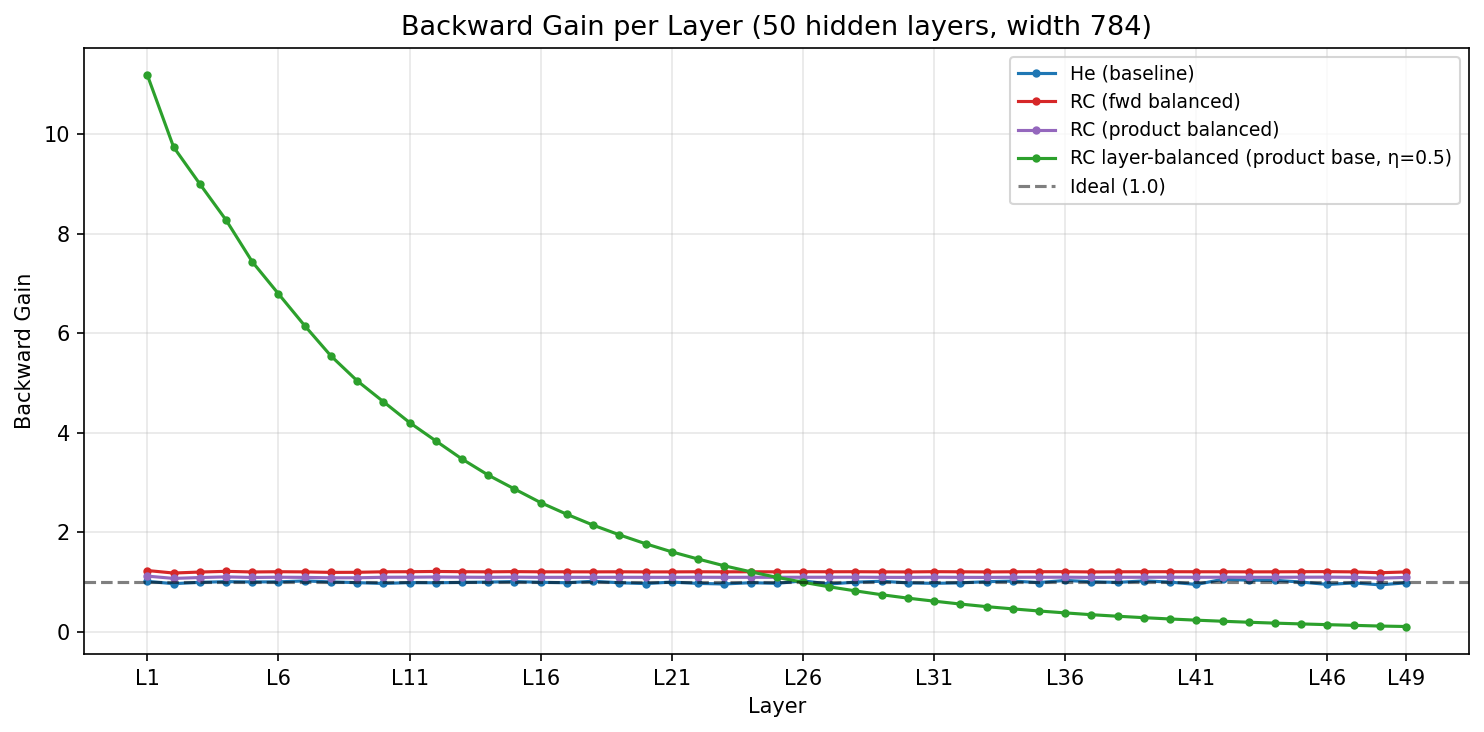
\includegraphics[width=0.95\textwidth]{figures/backward_gain.png}
  \caption{Backward gain per layer.  He and product-balanced both sit
           near 1.0 (He at 1.00, product at 1.10).  Fwd-balanced
           (red) is elevated at $\approx\!1.21$.}
  \label{fig:bwd-gain}
\end{figure}

\subsection{Gain product per layer}

\begin{figure}[H]
  \centering
  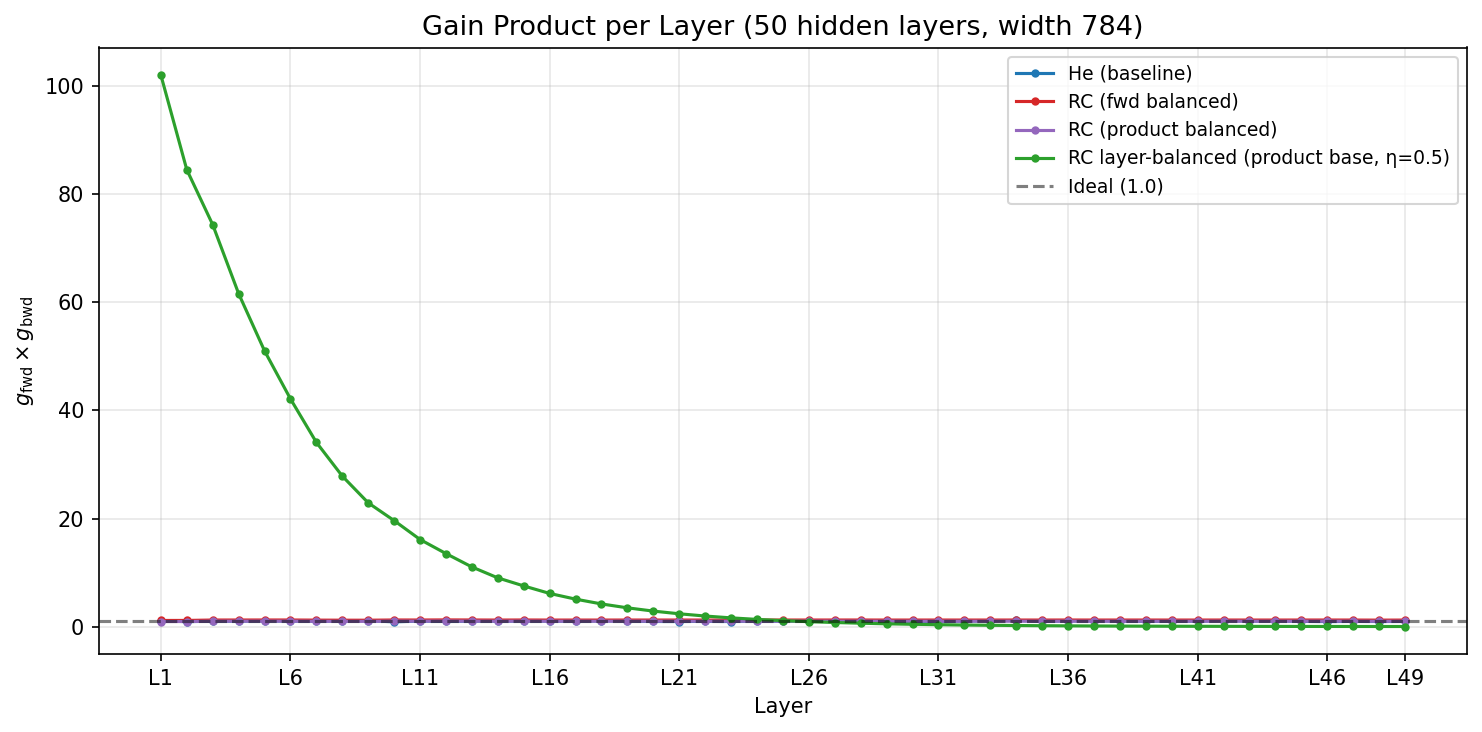
\includegraphics[width=0.95\textwidth]{figures/gain_product.png}
  \caption{Gain product $g_{\mathrm{fwd}} \times g_{\mathrm{bwd}}$ per
           layer.  \textbf{Product-balanced sits at 1.0} (the design target).
           He also sits at $\sim\!1.0$ (both gains individually $\approx 1$).
           Fwd-balanced sits at $\sim\!1.21$ (product $> 1$).}
  \label{fig:gain-product}
\end{figure}


%======================================================================
\section{Geometry Preservation (k-NN Accuracy)}
\label{sec:geometry}

\subsection{Setup}
Fashion-MNIST, 2000 samples, depths $L \in \{5, 10, 15, 20\}$,
square projections (width = input dim = 784).  k-NN accuracy ($k=5$)
measures whether class structure survives the projection.

\subsection{Results}

\begin{table}[H]
\centering
\caption{k-NN accuracy vs.\ depth.  Chance level = 0.10 (10 classes).}
\label{tab:knn}
\begin{tabular}{l c c c c}
\toprule
Initializer & 5\,L & 10\,L & 15\,L & 20\,L \\
\midrule
He (baseline)          & 0.829 & 0.800 & 0.784 & \textbf{0.752} \\
RC fwd-balanced        & 0.810 & 0.636 & 0.356 & 0.270 \\
RC product-balanced    & 0.810 & 0.636 & 0.356 & 0.269 \\
\bottomrule
\end{tabular}
\end{table}

\begin{figure}[H]
  \centering
  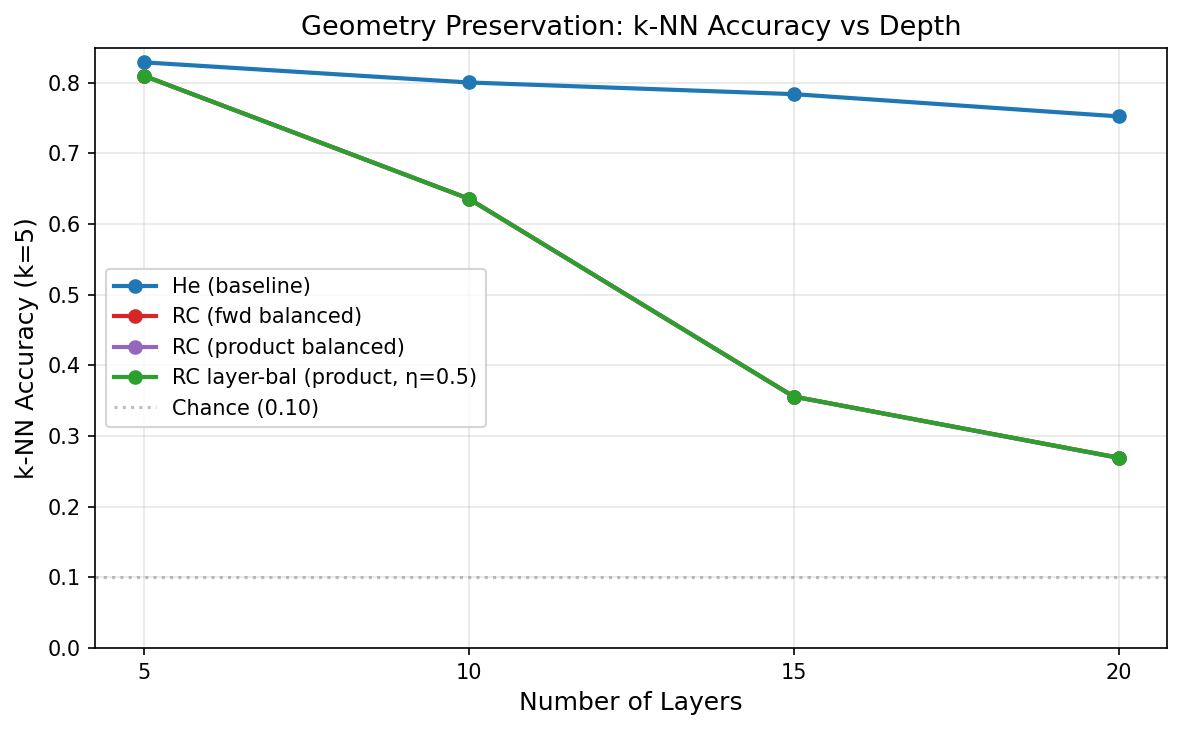
\includegraphics[width=0.7\textwidth]{figures/knn_accuracy.png}
  \caption{k-NN accuracy vs.\ depth.  He degrades gracefully (0.83 $\to$ 0.75).
           Both RC variants collapse identically to 0.27 by 20 layers.}
  \label{fig:knn}
\end{figure}

\begin{warnbox}
Product-balanced and fwd-balanced produce \textbf{identical geometry} at
every depth.  This is expected: both are fully row-centered
($\sum_j W_{ij} = 0$), so the DC-blindness that destroys class structure
is identical.  The variance only affects gain magnitudes, not the structural
constraint.  \textbf{No row-centered initialization can preserve geometry
at depth.}
\end{warnbox}


%======================================================================
\section{The Pareto Frontier: A Fundamental Limitation}
\label{sec:pareto}

\subsection{Theorem}

We now prove that the layer-balanced scheme (per-layer variance scaling) has
a fundamental depth-dependent limitation.

\begin{theorem}[Pareto budget]
  \label{thm:pareto}
  For row-centered initialization with per-layer scaling
  $s_\ell = s^{\ast} \cdot r^{\,\eta\,(\ell - (L+1)/2)}$, define:
  \begin{itemize}[nosep]
    \item Gradient ratio: $G(\eta) = r^{-(1-\eta)(L-1)}$
          \quad (max/min gradient across layers)
    \item Variance ratio: $V(\eta) = r^{-\eta(L-1)}$
          \quad (max/min weight variance across layers)
  \end{itemize}
  Then:
  \begin{equation}\label{eq:pareto}
    \boxed{\;G(\eta) \cdot V(\eta) = r^{-(L-1)} \quad\text{for all } \eta.\;}
  \end{equation}
  This product is \textbf{independent of $\eta$} and grows exponentially
  with depth.
\end{theorem}

\begin{proof}
  \begin{align*}
    G(\eta) \cdot V(\eta)
    &= r^{-(1-\eta)(L-1)} \cdot r^{-\eta(L-1)} \\
    &= r^{-(1-\eta)(L-1) - \eta(L-1)} \\
    &= r^{-(L-1)\bigl[(1-\eta) + \eta\bigr]} \\
    &= r^{-(L-1)}.
  \end{align*}
\end{proof}

\subsection{Numerical consequences}

\begin{table}[H]
\centering
\caption{Pareto budget $r^{-(L-1)}$ at various depths.}
\label{tab:budget}
\begin{tabular}{c c l}
\toprule
Depth $L$ & Budget $r^{-(L-1)}$ & Interpretation \\
\midrule
10  & $5.6\times$       & Manageable \\
20  & $38\times$         & Workable ($\eta = 0.75$ gives grad $= 2.5\times$, var $= 15\times$) \\
50  & $11{,}943\times$   & Severe (no $\eta$ makes both $< 110\times$) \\
100 & $1.7 \times 10^8$  & Catastrophic \\
\bottomrule
\end{tabular}
\end{table}

\subsection{Depth-adaptive $\eta$: the recipe}

Given a target gradient ratio~$T$, the required $\eta$ is:
\begin{equation}\label{eq:eta-adaptive}
  \eta^{\ast}(L, T) = \max\!\left(0,\; 1 - \frac{\ln T}{(L-1) \cdot \ln(1/r)}\right).
\end{equation}

\begin{table}[H]
\centering
\caption{Depth-adaptive $\eta$ for target gradient ratio $T = 10\times$.}
\label{tab:adaptive}
\begin{tabular}{c c c c}
\toprule
$L$ & $\eta^{\ast}$ & Gradient ratio & Variance ratio \\
\midrule
10  & 0.000 & $5.6\times$  & $1.0\times$ \\
20  & 0.368 & $10\times$   & $3.8\times$ \\
50  & 0.755 & $10\times$   & $1{,}194\times$ \\
100 & 0.879 & $10\times$   & $17{,}276{,}021\times$ \\
\bottomrule
\end{tabular}
\end{table}

At $L = 50$, achieving gradient ratio $\leq 10\times$ requires variance
ratio $\geq 1{,}194\times$.  The weight std at layer~1 would be
$\sim\!2.9$ (numerically feasible for float32) but the extreme scale
difference between layers creates practical training difficulties.

\begin{warnbox}
For $L \geq 50$, \textbf{no row-centered per-layer variance schedule can
simultaneously achieve gradient uniformity and bounded weight magnitudes}.
The exponential Pareto budget $r^{-(L-1)}$ is the fundamental barrier.
This is an intrinsic property of row centering + ReLU, not an artifact
of the specific scheme.
\end{warnbox}


%======================================================================
\section{Conclusion}
\label{sec:conclusion}

\subsection{What we proved}

\begin{enumerate}
  \item The product-balanced variance $v^{\ast} = 2\sqrt{\pi/(\pi-1)}/d
        \approx 2.422/d$ is the unique solution to
        $g_{\mathrm{fwd}} \cdot g_{\mathrm{bwd}} = 1$.  Empirically
        verified to 0.2\% accuracy.

  \item The Pareto budget theorem: for any row-centered per-layer scheme,
        $\text{gradient\_ratio} \times \text{variance\_ratio} = r^{-(L-1)}$.
        This budget grows exponentially with depth and cannot be reduced.

  \item Geometry experiments confirm that \textbf{all} row-centered variants
        (product-balanced, fwd-balanced, var-adj) destroy class structure
        identically.  The variance choice is irrelevant for geometry.
\end{enumerate}

\subsection{Implications for the thesis}

The product-balanced initializer is theoretically clean but does not solve
the core problem.  For deep networks ($L \geq 50$):

\begin{itemize}
  \item \textbf{Gradient stability} requires escaping the Pareto frontier,
        which means \emph{abandoning full row centering}.  Partial centering,
        orthogonal initialization, or fundamentally different structural
        constraints are needed.

  \item \textbf{Geometry preservation} is impossible with row centering at
        depth, regardless of variance.  The DC-blindness that defines row
        centering is the same mechanism that destroys class structure.

  \item The product-balanced variance remains useful as an \textbf{analytical
        tool}: it identifies the midpoint of the gain space and provides the
        natural base for any per-layer scheme at moderate depth ($L \leq 20$).
\end{itemize}

\end{document}
